\renewcommand{\theequation}{\theenumi}
\renewcommand{\thefigure}{\theenumi}
\begin{enumerate}[label=\thesection.\arabic*.,ref=\thesection.\theenumi]
\numberwithin{equation}{enumi}
\numberwithin{figure}{enumi}

\item Two students are solving the same problem independently,if the probability of first one solves the problem is $\frac{3}{5}$ and the probability that the second one solves the problem is $\frac{4}{5}$ ,what is the probability that atleast one of them solves the problem?
\begin{enumerate}

\item $ \frac{17}{25}$\\
\item $\frac{19}{25}$\\
\item $ \frac{21}{25}$\\
\item $\frac{23}{25}$

\end{enumerate}
%
\solution
Let X,Y be two events representing solving the problem by students A,B respectively.\\
Given 
\begin{align}
    \pr{X}=\frac{3}{5}\label{june2018-18:eq:0.0.1}\\
    \pr{Y}=\frac{4}{5}\label{june2018-18:eq:0.0.2}
\end{align}
Since students solve the problem independently,So events X and Y are independent,
For independent events
\begin{align}
    \pr{XY}&=\pr{X}\times \pr{Y}
\intertext{from \eqref{june2018-18:eq:0.0.1} and \eqref{june2018-18:eq:0.0.2}}
    \pr{XY}&=\frac{3}{5}\times \frac{4}{5}\\
    \pr{XY}&=\frac{12}{25}\label{june2018-18:eq:0.0.5}
\end{align}
\\
\\Now we have to find probability of solving the problem by atleast one of them i.e $\pr{X+Y}$.\\
As,
\begin{align}
    \pr{X+Y}&=\pr{X}+\pr{Y}-\pr{XY}\\
\intertext{from \eqref{june2018-18:eq:0.0.1}, \eqref{june2018-18:eq:0.0.2}, \eqref{june2018-18:eq:0.0.5}}
\pr{X+Y}&=\frac{3}{5}+\frac{4}{5}-\frac{12}{25}\\
\pr{X+Y}&=\frac{23}{25}
\end{align}
Hence the required probability is $\frac{23}{25}$
%
\item A standard fair die is rolled until some face other than 5 or 6 turns up.Let X denote the face value of the last roll.Let A=\{X is even\} and B=\{X is atmost 2\}
Then,
\begin{enumerate}
\begin{multicols}{2}
\setlength\itemsep{1em}
\item $\Pr{(A\cap {B})}=0$\\
\item $\Pr{(A \cap B)}=\frac{1}{6}$\\
\item $\Pr{(A\cap B)}=\frac{1}{4}$\\
\item $\Pr{({A} \cap {B})}=\frac{1}{3}$
\end{multicols}
\end{enumerate}
%
\solution
\begin{figure}[h!]
    \caption{Markov chain}
    \resizebox{\columnwidth}{!}{%
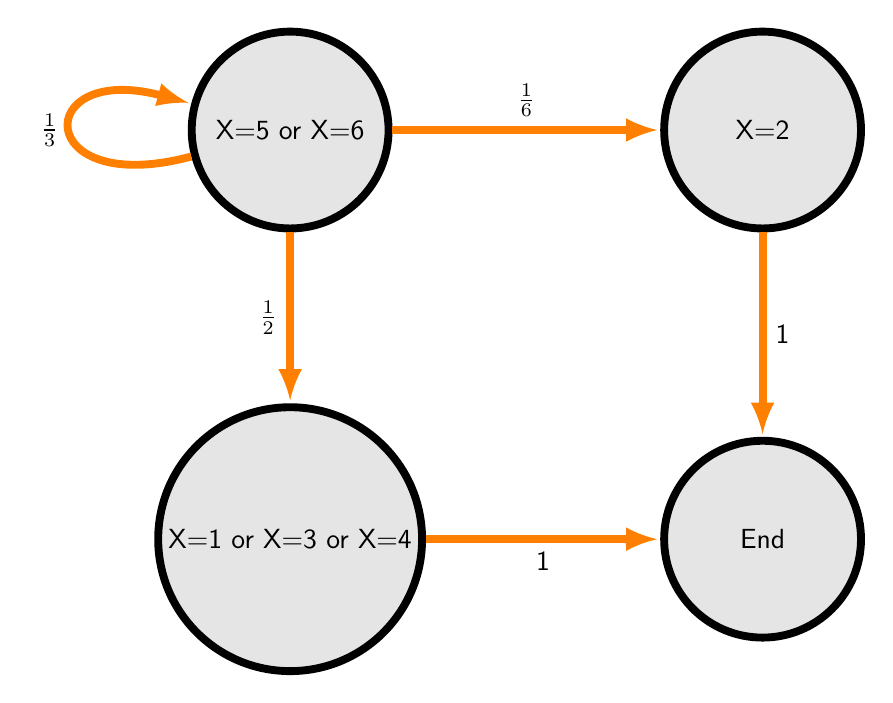
\begin{tikzpicture}[font=\sffamily]
        % Setup the style for the states
        \tikzset{node style/.style={state, 
                                    minimum width=2.5cm,
                                    line width=1mm,
                                    fill=gray!20!white}}
        % Draw the states
        \node[node style] at (0, 0)     (A)     {X=5 or X=6};
        \node[node style] at (6, 0)     (B)     {X=2};
        \node[node style] at (6, -5.196) (end) {End};
        \node[node style] at (0, -5.196) (C) {X=1 or X=3 or X=4};
        % Connect the states with arrows
        \draw[every loop,
              auto=right,
              line width=1mm,
              >=latex,
              draw=orange,
              fill=orange]
              (A) edge[bend left=0] node {$\frac{1}{2}$} (C)
              (C) edge[bend left=0] node {1} (end)
              (A) edge[loop left] node {$\frac{1}{3}$} (A)
            (A)     edge[bend right=0, auto=left] node {$\frac{1}{6}$} (B)
            (B)     edge[bend left=0, auto=left] node {1} (end);
    \end{tikzpicture}
    }
    \end{figure}
Let us assume the following table.
\begin{table}[h!]
\centering
\caption{}
\label{june2018-49:table:1}
\resizebox{\columnwidth}{!}{%
\begin{tabular}{|c|c|c|c|}
    \hline
    state 1&state 2 &state 3 &state 4\\
    \hline
$X=5$ or $X=6$&$X=2$&$X=1$ or $X=3$ or $X=4$ &end \\    
    \hline
\end{tabular}}
\end{table}
Let us represent the markov chain diagram in a matrix.Let $P_{ij}$ represent the element of a matrix which is in $i^{th}$ row and $j^{th}$ column.The value of $P_{ij}$ is equal to probability of transition from state $i$ to state $j$
\begin{equation}
P=\begin{bmatrix}
\frac{1}{3}&\frac{1}{6}&\frac{1}{2}&0\\
0&0&0&1\\
0&0&0&1\\
0&0&0&0\\
\end{bmatrix}
\end{equation}
We need the probability that $X=2$.Hence required probability is
\begin{equation}
    P_{12}+(P_{12})^{2}+\cdots+\infty \label{june2018-49:eq:reqprob}
\end{equation}
where $P_{12}^{n}$ represents the 1st row ,2nd column element in the $P^{n}$
\begin{align}
P^2&=\begin{bmatrix}
\frac{1}{3}&\frac{1}{6}&\frac{1}{2}&0\\
0&0&0&1\\
0&0&0&1\\
0&0&0&0\\
\end{bmatrix} \times
\begin{bmatrix}
\frac{1}{3}&\frac{1}{6}&\frac{1}{2}&0\\
0&0&0&1\\
0&0&0&1\\
0&0&0&0\\
\end{bmatrix}\\
&=\begin{bmatrix}
\frac{1}{9}&\frac{1}{18}&\frac{1}{6}&0\\
0&0&0&0\\
0&0&0&0\\
0&0&0&0\\
\end{bmatrix}
\end{align}
\begin{align}
    P^3&=(P^2)(P^1)\\
    &=\begin{bmatrix}
\frac{1}{9}&\frac{1}{18}&\frac{1}{6}&0\\
0&0&0&0\\
0&0&0&0\\
0&0&0&0\\
\end{bmatrix}\times
\begin{bmatrix}
\frac{1}{3}&\frac{1}{6}&\frac{1}{2}&0\\
0&0&0&1\\
0&0&0&1\\
0&0&0&0\\
\end{bmatrix}\\
&=\begin{bmatrix}
\frac{1}{27}&\frac{1}{54}&\frac{1}{18}&0\\
0&0&0&0\\
0&0&0&0\\
0&0&0&0\\
\end{bmatrix}
\end{align}
From above we can notice that each time $P_{12}$ reduces by $\frac{1}{3}$.Hence from \eqref{june2018-49:eq:reqprob},
\begin{equation}
    \sum_{i=0}^{\infty}\brak{\frac{1}{3}}^i \frac{1}{6}
\end{equation}
From Geometric progression we can write ,required probability =$\frac{1}{4}$
$\therefore$ \textbf{option C is correct}
%
\item Let X and Y be two random variables with joint probability density function
\begin{align*}
    f(x.y)=
    \begin{cases}
    \cfrac{1}{\pi} & 0\le x^2 + y^2 \le 1\\
    0 & otherwise
    \end{cases}
\end{align*}
Which of the following statements are correct?
\begin{enumerate}
    \item
    X and Y are independent.
    
    \item
    $\pr{X>0}=\cfrac{1}{2}$
    
    \item
    E(Y)=0
    
    \item
    Cov(X,Y)=0
\end{enumerate}
%
%
\solution
%\begin{figure}[h!]
    \caption{Markov chain}
    \resizebox{\columnwidth}{!}{%
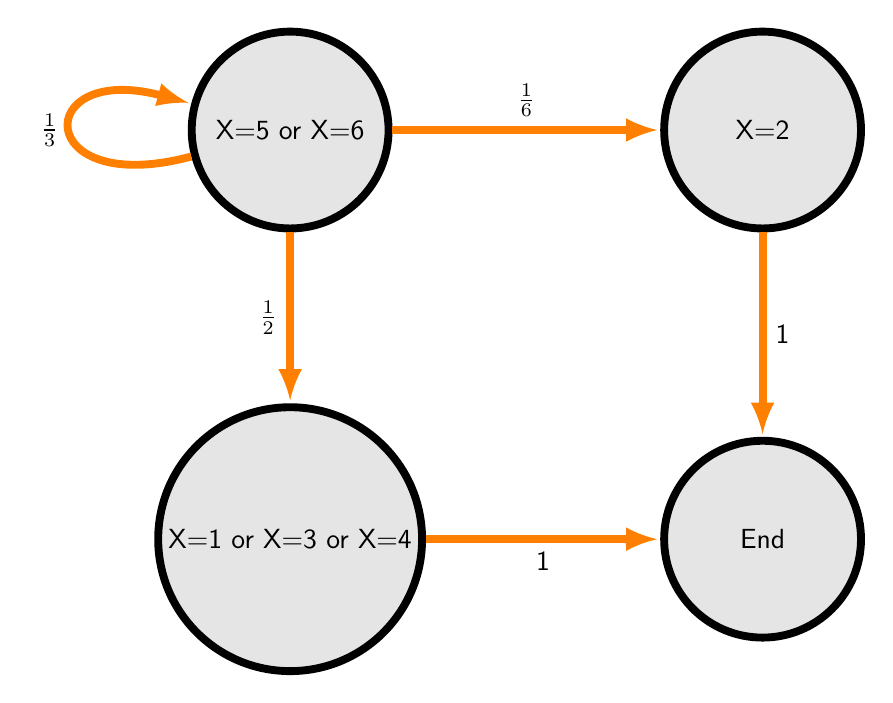
\begin{tikzpicture}[font=\sffamily]
        % Setup the style for the states
        \tikzset{node style/.style={state, 
                                    minimum width=2.5cm,
                                    line width=1mm,
                                    fill=gray!20!white}}
        % Draw the states
        \node[node style] at (0, 0)     (A)     {X=5 or X=6};
        \node[node style] at (6, 0)     (B)     {X=2};
        \node[node style] at (6, -5.196) (end) {End};
        \node[node style] at (0, -5.196) (C) {X=1 or X=3 or X=4};
        % Connect the states with arrows
        \draw[every loop,
              auto=right,
              line width=1mm,
              >=latex,
              draw=orange,
              fill=orange]
              (A) edge[bend left=0] node {$\frac{1}{2}$} (C)
              (C) edge[bend left=0] node {1} (end)
              (A) edge[loop left] node {$\frac{1}{3}$} (A)
            (A)     edge[bend right=0, auto=left] node {$\frac{1}{6}$} (B)
            (B)     edge[bend left=0, auto=left] node {1} (end);
    \end{tikzpicture}
    }
    \end{figure}
Let us assume the following table.
\begin{table}[h!]
\centering
\caption{}
\label{june2018-49:table:1}
\resizebox{\columnwidth}{!}{%
\begin{tabular}{|c|c|c|c|}
    \hline
    state 1&state 2 &state 3 &state 4\\
    \hline
$X=5$ or $X=6$&$X=2$&$X=1$ or $X=3$ or $X=4$ &end \\    
    \hline
\end{tabular}}
\end{table}
Let us represent the markov chain diagram in a matrix.Let $P_{ij}$ represent the element of a matrix which is in $i^{th}$ row and $j^{th}$ column.The value of $P_{ij}$ is equal to probability of transition from state $i$ to state $j$
\begin{equation}
P=\begin{bmatrix}
\frac{1}{3}&\frac{1}{6}&\frac{1}{2}&0\\
0&0&0&1\\
0&0&0&1\\
0&0&0&0\\
\end{bmatrix}
\end{equation}
We need the probability that $X=2$.Hence required probability is
\begin{equation}
    P_{12}+(P_{12})^{2}+\cdots+\infty \label{june2018-49:eq:reqprob}
\end{equation}
where $P_{12}^{n}$ represents the 1st row ,2nd column element in the $P^{n}$
\begin{align}
P^2&=\begin{bmatrix}
\frac{1}{3}&\frac{1}{6}&\frac{1}{2}&0\\
0&0&0&1\\
0&0&0&1\\
0&0&0&0\\
\end{bmatrix} \times
\begin{bmatrix}
\frac{1}{3}&\frac{1}{6}&\frac{1}{2}&0\\
0&0&0&1\\
0&0&0&1\\
0&0&0&0\\
\end{bmatrix}\\
&=\begin{bmatrix}
\frac{1}{9}&\frac{1}{18}&\frac{1}{6}&0\\
0&0&0&0\\
0&0&0&0\\
0&0&0&0\\
\end{bmatrix}
\end{align}
\begin{align}
    P^3&=(P^2)(P^1)\\
    &=\begin{bmatrix}
\frac{1}{9}&\frac{1}{18}&\frac{1}{6}&0\\
0&0&0&0\\
0&0&0&0\\
0&0&0&0\\
\end{bmatrix}\times
\begin{bmatrix}
\frac{1}{3}&\frac{1}{6}&\frac{1}{2}&0\\
0&0&0&1\\
0&0&0&1\\
0&0&0&0\\
\end{bmatrix}\\
&=\begin{bmatrix}
\frac{1}{27}&\frac{1}{54}&\frac{1}{18}&0\\
0&0&0&0\\
0&0&0&0\\
0&0&0&0\\
\end{bmatrix}
\end{align}
From above we can notice that each time $P_{12}$ reduces by $\frac{1}{3}$.Hence from \eqref{june2018-49:eq:reqprob},
\begin{equation}
    \sum_{i=0}^{\infty}\brak{\frac{1}{3}}^i \frac{1}{6}
\end{equation}
From Geometric progression we can write ,required probability =$\frac{1}{4}$
$\therefore$ \textbf{option C is correct}
%
\item Let X and Y be two random variables with joint probability density function
\begin{align*}
    f(x.y)=
    \begin{cases}
    \cfrac{1}{\pi} & 0\le x^2 + y^2 \le 1\\
    0 & otherwise
    \end{cases}
\end{align*}
Which of the following statements are correct?
\begin{enumerate}
    \item
    X and Y are independent.
    
    \item
    $\pr{X>0}=\cfrac{1}{2}$
    
    \item
    E(Y)=0
    
    \item
    Cov(X,Y)=0
\end{enumerate}
%
%
\solution
\begin{enumerate}
    \item 
The marginal PDF of X is given by
\begin{align}
    f_X(x)&=\displaystyle\int\limits_{y=-\infty}^{y=\infty} f_{XY}(x,y) dy\\
          &=\displaystyle\int\limits_{y=-\sqrt{1-x^2}}^{y=\sqrt{1-x^2}}\cfrac{1}{\pi} dy\\
          &=\cfrac{2\sqrt{1-x^2}}{\pi}
\end{align}
The marginal PDF of Y is given by
\begin{align}
    f_Y(x)&=\displaystyle\int\limits_{x=-\infty}^{x=\infty} f_{XY}(x,y) dx\\
          &=\displaystyle\int\limits_{x=-\sqrt{1-y^2}}^{x=\sqrt{1-y^2}}\cfrac{1}{\pi} dx\\
          &=\cfrac{2\sqrt{1-y^2}}{\pi}
\end{align}
Now,
\begin{align}
    f_X(x)\times f_Y(x) &=\cfrac{2\sqrt{1-x^2}}{\pi} \times\cfrac{2\sqrt{1-y^2}}{\pi}\\
    &= \cfrac{4(1-x^2)(1-y^2)}{\pi^2}\\
    &\neq \cfrac{1}{\pi}\\
    &\neq f_{XY}(x,y)
\end{align}
Therefore, X and Y are not independent.\\
\item
Now,
\begin{align}
    \pr{X>0}&=\displaystyle\int\limits_{x=0}^{x=\infty}f_X(x)dx\\
    &=\displaystyle\int\limits_{x=0}^{x=1}\cfrac{2\sqrt{1-x^2}}{\pi} dx\\
    &=\brak{\frac{\arcsin{(x)}+x\sqrt{1-x^2}}{\pi}}_{0}^{1}\\
    &=\cfrac{1}{2}
\end{align}
Therefore, option(2) is correct.\\
\item
Now,
\begin{align}
    E\sbrak{Y}&=\displaystyle\int\limits_{y=-\infty}^{y=\infty}yf_Y(y)dy\\
    &=\displaystyle\int\limits_{y=-1}^{y=1}\cfrac{2y\sqrt{1-y^2}}{\pi}dy\\
    &=\brak{\frac{-2(1-y^2)^{\frac{3}{2}}}{3\pi}}_{-1}^{1}\\
    &=0
\end{align}
Therefore, option(3) is also correct.\\
\item
Now,
\begin{align}
    E\sbrak{XY}&=\displaystyle\int\limits_{x}\displaystyle\int\limits_{y}xyf_{XY}(x,y)dydx\\
    &=\displaystyle\int\limits_{x=-1}^{x=1}\displaystyle\int\limits_{y=-\sqrt{1-x^2}}^{y=\sqrt{1-x^2}}\cfrac{xy}{\pi}dydx\\
    &=\cfrac{x}{\pi} \displaystyle\int\limits_{x=-1}^{x=1}\brak{\cfrac{y^2}{2}}_{-\sqrt{1-x^2}}^{\sqrt{1-x^2}}dx\\
    &=0
\end{align}
Now,
\begin{align}
    Cov(X,Y)&=E\sbrak{XY}-E\sbrak{X}E\sbrak{Y}\\
    &=0-E\sbrak{X}\times0\\
    &=0
\end{align}
Therefore, option(4) is also correct.\\
\end{enumerate}
%
\item A simple random variable of size n will be drawn from a class of 125 students, and the mean mathematics score of the sample will be computed, If the standard error of the sample mean for "with replacement sampling" is twice as much as the standard error of the sample mean for "without replacement sampling", the value of n is ? 
	\begin{enumerate}
	\item 32
	\item 63
	\item 79
	\item 94
	\end{enumerate}
%
\solution
Let N be the population size so, N=120. The given sample size is n.
\textbf{Notations :}
y : student under consideration.
$y_i$ : Maths marks of $i^{th}$ student in the sample.
Y : student of class.
$Y_i$ : Maths marks of $i^{th}$ student in the class.
$\overline{y}=\dfrac{1}{n}\sum_{i=1}^{n}y_i$ : Average of sample class.
$\overline{Y}=\dfrac{1}{N}\sum_{i=1}^{N}Y_i$ : Average of whole class.
$S^2 = \dfrac{1}{N-1} \sum_{i=1}^{N} (Y_i-\bar{Y})^2$ : S=Std dev of the class.
$\sigma^2=\dfrac{1}{N} \sum_{i=1}^{N} (Y_i-\bar{Y})^2$ : Variance of the class.
Standard error of sample mean $SE_{mean}=\dfrac{s}{\sqrt{n}}$.\\
Where 
\begin{align*}
s & = \text{standard deviation of sample mean.}\\
n & = \text{sample class size.}
\end{align*}
\textbf{Variance of the $\overline{y}$}
\begin{align}
& V(\overline{y})= E(\overline{y}-\overline{Y})^2\\
& = E\left[\dfrac{1}{n} \sum_{i=1}^{n}(y_i-\overline{Y})\right]^2\\
& = E\left[\dfrac{1}{n^2} \sum_{i=1}^{n} (y_i-\overline{Y})^2 + \dfrac{1}{n^2} \underset{1\leq i\neq j\leq n}{\sum\sum}\, (y_i-\overline{Y})(y_j-\overline{Y})\right]\\
& = \dfrac{1}{n^2}\sum_{i=1}^{n} E(y_i-\overline{Y})^2+\dfrac{1}{n^2} \underset{1\leq i\neq j\leq n}{\sum\sum}\, E(y_i-\overline{Y})(y_j-\overline{Y})\\
& \text{Let } K=\underset{1\leq i\neq j\leq n}{\sum\sum}\, E(y_i-\overline{Y})(y_j-\overline{Y})\\
& = \dfrac{1}{n^2}\sum_{i=1}^{n} \sigma^2 + \dfrac{K}{n^2}\\
& = \dfrac{1}{n^2} n \sigma^2 +\dfrac{K}{n^2}\\
& = \dfrac{N-1}{Nn} S^2+\dfrac{K}{n^2}\label{june2018-58:eq_1}
\end{align}
Finding the value of K in case of Simple random sampling with repetition (SRSWR)and Simple random sampling without repetition(SRSWOR) allows us to calculate the variance of mean.
\vspace{0.5 cm}
\textbf{K value in case of SRSWOR}
\begin{align*}
&K=\underset{1\leq i\neq j\leq n}{\sum\sum}\, E(y_i-\overline{Y})(y_j-\overline{Y})
\end{align*}
Consider
\begin{multline*}
E(y_i-\overline{Y})(y_j-\overline{Y})= \\
\dfrac{1}{N(N-1)}\underset{1\leq k\neq l\leq n}{\sum\sum}\, E(y_k-\overline{Y})(y_l-\overline{Y})
\end{multline*}
Since
\begin{multline*}
\left[\sum_{k=1}^N(y_k-\overline{Y})\right]^2=\sum_{i=1}^{N}(y_k-\overline{Y})^2+\\
\underset{1\leq k\neq l\leq n}{\sum\sum}\, E(y_k-\overline{Y})(y_l-\overline{Y})
\end{multline*}
\begin{align*}
&\implies 0 = (N-1)S^2+\underset{1\leq k\neq l\leq n}{\sum\sum}\, E(y_k-\overline{Y})(y_l-\overline{Y})\\
& \implies E(y_i-\overline{Y})(y_j-\overline{Y})=\dfrac{1}{N(N-1)}(N-1)(-S^2)\\
& \implies K = n(n-1)\dfrac{(-S^2)}{N}
\end{align*}
Putting this value in (\ref{june2018-58:eq_1}) gives us 
\begin{align}
V(\overline{y})_{WOR} & = \dfrac{N-1}{Nn} S^2+ \dfrac{n-1(-S^2)}{Nn}\\
& = \dfrac{N-n}{Nn} S^2 \label{june2018-58:eq_2}
\end{align}
\textbf{K value in case of SRSWR}
\begin{align*}
&K=\underset{1\leq i\neq j\leq n}{\sum\sum}\, E(y_i-\overline{Y})(y_j-\overline{Y})
\end{align*}
Since we are selecting the samples with replacements choosing $i^{th}$ and $j^{th}$ sample is independent of each other. So,
\begin{align*}
K&=\underset{1\leq i\neq j\leq n}{\sum\sum}\, E(y_i-\overline{Y})E(y_j-\overline{Y})\\
& = 0\\
& \text{(Since deviation about mean is 0)}
\end{align*}
Putting K=0 in (\ref{june2018-58:eq_1}) we get 
\begin{align}
V(\overline{y})_{WR} & = \dfrac{N-1}{Nn} S^2\label{june2018-58:eq_3}
\end{align}
From equation \eqref{june2018-58:eq_2}  standard error of mean of sample class without repetition
\begin{align}
{SE}_{WOR} & = \dfrac{s}{\sqrt{n}}\\
& = \sqrt{\dfrac{V(\overline{y})_{WOR}}{n}}\\
& = \sqrt{\dfrac{N-n}{Nn^2}}S \label{june2018-58:eq_4}
\end{align} 
From equation \eqref{june2018-58:eq_3}  standard error of mean of sample class with repetition
\begin{align}
{SE}_{WR} & = \sqrt{\dfrac{V(\overline{y})_WR}{n}}\\
& = \sqrt{\dfrac{N-1}{Nn^2}}S \label{june2018-58:eq_5}
\end{align}
Given to find the value of n if $2 \times {SE}_{WOR} =  {SE}_{WR}$.
From \eqref{june2018-58:eq_4} and \eqref{june2018-58:eq_5} we can write 
\begin{align}
& 2\sqrt{\dfrac{N-n}{Nn^2}}S= \sqrt{\dfrac{N-1}{Nn^2}}S\\
\implies & 4(N-n) = N-1\\
\implies & 4N+1-N=4n\\
\implies & 4n=3(125)+1\\
\implies & n=94
\end{align}
Therefore the sample size for the given condition to be met is n=94.(\textbf{Option D})



\item Let X and Y be two independent and identically distributed (I.I.D) random variables uniformly distributed in (0,1). Let $Z = max(X,Y)$ and $W = min(X,Y)$ , then the probability that $[Z-W >\frac{1}{2}]$ is\\
\\(A) $\frac{1}{2}$\\
\\(B) $\frac{3}{4}$\\
\\(C) $\frac{1}{4}$\\
\\(D) $\frac{2}{3}$    
%
\solution

X and Y are two independent random variables. \\
Let
\begin{align}
    f_X\brak{x} &= \Pr\brak{X=x} \\
    f_Y\brak{y} &= \Pr\brak{Y=y}  \\
    f_V\brak{v} &= \Pr\brak{V=v}
\end{align}
be the probability densities of random variables X ,Y and V=X-Y.\\
The density for X is \\
\begin{align}
\label{june2018-50eq:_pdf_x}
f_{X}(x)  = 
\begin{cases}
1 & 0 \le x \le 1
\\
0 & otherwise
\end{cases}
\end{align}
We have ,
\begin{equation}
    V= X-Y \iff v= x- y \iff x = v+y
\end{equation}
The density of X can also be represented as,
\begin{align}
\label{june2018-50eq:pdf_x}
f_{X}(v+y)  = 
\begin{cases}
1 & 0 \le v+y \le 1
\\
0 & otherwise
\end{cases}
\end{align}
and the density of Y is,
\begin{align}
\label{june2018-50eq:pdf_y}
f_{Y}(y)  = 
\begin{cases}
1 & 0 \le y \le 1
\\
0 & otherwise
\end{cases}
\end{align}
The density of V i.e. $V=X-Y $ is given by the convolution of $f_X(-v)$ with $f_Y(v)$.
\begin{equation}
    f_V(v) =  \int_{- \infty}^{\infty} f_X(v+y)f_Y(y) \,dy 
\end{equation}
From \ref{june2018-50eq:pdf_x} and \ref{june2018-50eq:pdf_y} we have, \\
The integrand is 1 when,
\begin{align}
    0 \le y \le 1 \\
    0 \le v+y \le 1 \\
    -v \le y \le 1-v
\end{align}
and zero, otherwise. \\
Now when $-1 \le v \le 0$ we have, 
\begin{align}
    f_V(v) &=   \int_{-v}^{1} \,dy  \\
          &= (1 - (-v)) \\
          &= 1+v
\end{align}

For $0 \le v \le 1$ we have, 
\begin{align}
    f_V(v) &=   \int_{0}^{1-v} \,dy  \\
          &= (1-v - (0)) \\
          &= 1-v
\end{align}

Therefore the density of V is given by
\begin{align}
\label{june2018-50eq:pdf_v}
f_{V}(v)  = 
\begin{cases}
1+v & -1 \le v \le 0
\\
1-v & 0 < v \le 1
\\
0 & otherwise
\end{cases}
\end{align}

The plot for PDF of $V $ can be observed at figure \ref{june2018-50fig:The PDF of V}
\begin{figure}[!ht]
       \centering
    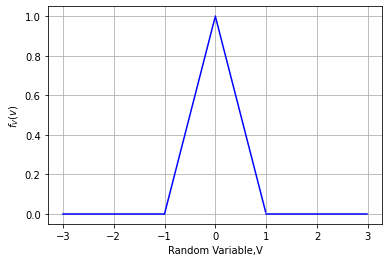
\includegraphics[width=\columnwidth] {solutions/2018/june/50/Assignment_3_Fig_1.png}
    \caption{The PDF of V}
    \label{june2018-50fig:The PDF of V}
\end{figure}

The CDF of V is defined as,
\begin{equation}
    F_V(v) = \Pr\brak{V \le v}
\end{equation}
Now for $ v \le 0 $,
 \begin{align}
    \Pr\brak{V\le v} &=  \int_{-\infty}^{v}f_{V}(v) \,dv  \\
          &=  \int_{-1}^{v} (1+v) \,dv  \\
          &=  \left(\dfrac{v^2}{2}+v \right) \Biggr|_{-1}^{v}  \\
          &=   \left(\left(\dfrac{v^2}{2}+v \right) - \left(\dfrac{1}{2} -1 \right)\right) \\
          &= \dfrac{v^2+2v +1}{2}
\end{align}
Similarly for $v \le 1$,
\begin{align}
    \Pr\brak{V\le v} &=  \int_{-\infty}^{v}f_{V}(v) \,dv  \\
          &=  \dfrac{1}{2} + \int_{0}^{v}(1-v)\,dz  \\
          &=  \dfrac{-v^2+2v+1}{2}
\end{align}

The CDF is as below: 
\begin{align}
\label{june2018-50eq:cdf_v}
F_{V}(v)  = 
\begin{cases}
0 & v < -1
\\
\dfrac{v^2+2v + 1}{2} &  v \le 0
\\
\dfrac{-v^2+2v+1}{2} &  v \le 1
\\
1 & v > 1
\end{cases}
\end{align}

The plot for CDF of $V $ can be observed at figure \ref{june2018-50fig:The CDF of V}\\

\begin{figure}[!ht]
       \centering
    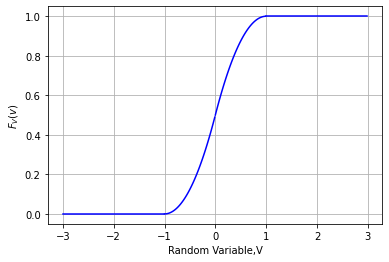
\includegraphics[width=\columnwidth] {solutions/2018/june/50/Assignment_3_Fig_2.png}
    \caption{The CDF of V}
    \label{june2018-50fig:The CDF of V}
\end{figure}

We need  $\pr{Z-W >\frac{1}{2}}$ where $Z = max(X,Y)$ and $W = min(X,Y)$. Now,

\begin{align}
\label{june2018-50eq:pdf_v}
Z-W  = 
\begin{cases}
X-Y & \text{for } X \geq Y
\\
Y-X & \text{for } X < Y
\end{cases}
\end{align}

Therefore,
\begin{align}
    \pr{Z-W >\frac{1}{2}} &= \pr{X-Y>\frac{1}{2},X \geq Y} \nonumber \\
    &+\pr{Y-X > \frac{1}{2}, X < Y}\\
    &= \pr{X-Y>\frac{1}{2}} +\pr{Y-X>\frac{1}{2}}\\
    &= \pr{V > \frac{1}{2}} + \pr{-V > \frac{1}{2}}\\
    &= 1 - \pr{V \leq \frac{1}{2}} + \pr{V < \frac{-1}{2}}\\
    &= 1-F_V(\frac{1}{2}) + F_V(-\frac{1}{2})\\
    &= 1 -\frac{7}{8} + \frac{1}{8}\\
    &= \frac{1}{4}
\end{align}

Hence the correct answer is option (C).




% \item Consider a Markov Chain with state space $S = \cbrak{1,2, 3}$ and transition matrix
% \begin{align}
% P = 
% \begin{blockarray}{c@{\hspace{1pt}}rrr@{\hspace{3pt}}}
%             & 1   & 2 & 3 \\
%         \begin{block}{r@{\hspace{3pt}}@{\hspace{1pt}}
%     (@{\hspace{1pt}}rrr@{\hspace{1pt}}@{\hspace{1pt}})}
%         1 &  0 & \frac{1}{2} & \frac{1}{2}   \\ [2mm]
%         2 & \frac{1}{2}  & 0 & \frac{1}{2}\\ [2mm]
%         3 & \frac{1}{2}  &  \frac{1}{2} & 0  \\ [2mm]
% %
%         \end{block}
%     \end{blockarray}
% \end{align}
% %
% Let $\vec{\pi}$ be a stationary distribution of the Markov chain and $d(1)$ denote the
% period of state 1.  Which of the following statements are correct?
% \begin{enumerate}
% \item $d(1) = 1$
% \item $d(1) = 2$
% \item $\pi_1 = \frac{1}{2}$
% \item $\pi_1 = \frac{1}{3}$
% \end{enumerate}
% \solution
% %
\begin{figure}
\begin{center}
\usetikzlibrary{automata, positioning}
    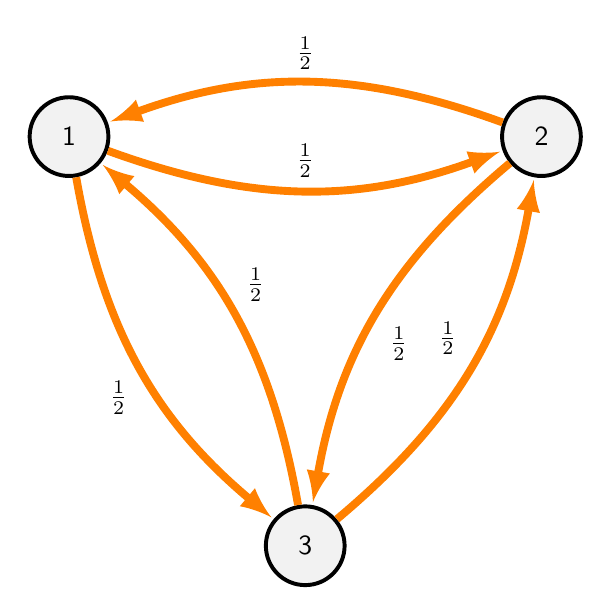
\begin{tikzpicture}[font=\sffamily]
        % Setup the style for the states
        \tikzset{node style/.style={state, 
                                    minimum width=1cm,
                                    line width=0.5mm,
                                    fill=gray!10!white}}

        % Draw the states
        \node[node style] at (0, 0)     (1)     {1};
        \node[node style] at (6, 0)     (2)     {2};
        \node[node style] at (3, -5.196) (3) 	{3};

        % Connect the states with arrows
        \draw[every loop,
              auto=right,
              line width=1mm,
              >=latex,
              draw=orange,
              fill=orange]
            (1)     edge[bend right=20]            node {$\frac{1}{2}$} (3)
            (1)     edge[bend right=20, auto=left] node {$\frac{1}{2}$} (2)
            (2)     edge[bend right=20]            node {$\frac{1}{2}$} (1)
            (2)     edge[bend right=20, auto=left] node {$\frac{1}{2}$} (3)
            (3) edge[bend right=20]            node {$\frac{1}{2}$} (1)
            (3) edge[bend right=20, auto=left] node {$\frac{1}{2}$} (2);
    \end{tikzpicture}  
    \caption{State transition diagram}
\end{center}
    \end{figure}    
    \begin{enumerate}
    \item{ The period of state 1 i.e, $d(1)$ is given as:
    \begin{align}
    d(1)=GCD\{n : P_{11}^n > 0\} \label{eq:solutions/2018/june/105/eq1a}
    \end{align}
     For $n=1$,
    \begin{align}
    \vec{P}=\myvec{0&\frac{1}{2}&\frac{1}{2}\\\frac{1}{2}&0&\frac{1}{2}\\\frac{1}{2}&\frac{1}{2}&0}\\
    \end{align}
    For $n=2$,
    \begin{align}
    \vec{P}^2=\myvec{\frac{1}{2}&\frac{1}{4}&\frac{1}{4}\\\frac{1}{4}&\frac{1}{2}&\frac{1}{4}\\\frac{1}{4}&\frac{1}{4}&\frac{1}{2}}\\
    \end{align}
    For $n=3$,
    \begin{align}
    \vec{P}^3=\myvec{\frac{1}{4}&\frac{3}{8}&\frac{3}{8}\\\frac{3}{8}&\frac{1}{4}&\frac{3}{8}\\\frac{3}{8}&\frac{3}{8}&\frac{1}{4}}\\
    \end{align}
        For $n=4$,
    \begin{align}
    \vec{P}^4=\myvec{\frac{3}{8}&\frac{5}{16}&\frac{5}{16}\\\frac{5}{16}&\frac{3}{8}&\frac{5}{16}\\\frac{5}{16}&\frac{5}{16}&\frac{3}{8}}
    \end{align}
Thus $P_{11}^n$ follows the sequence, that is defined as:
\begin{align}
    P_{11}^n= 
\begin{cases}
	0,& \text{if } n=1\\
    \frac{1}{2},& \text{if } n=2\\
    \frac{1}{2}(P_{11}^{n-1}+P_{11}^{n-2}),& \text{if } n >2
\end{cases}
\end{align}
    Since, for $n>1$, $P_{11}^n>0$
    \begin{align}
    d(1)=GCD\{2,3,4,5\cdots\}\\
    \therefore d(1)=1 \label{eq:solutions/2018/june/105/eq1}
    \end{align}
    Thus statement a is correct}\\
    \item{As calucalted above in \ref{eq:solutions/2018/june/105/eq1}, $d(1)=1$\\
    Thus statement b is incorrect.}\\
    \item{For stationary distribution,
    \begin{align}
    &\sum_{i=1}^{i=n} \pi_i = 1 \\
    &\implies\myvec{1&1&1}\myvec{\pi_1\\\pi_2\\\pi_3}=1\label{eq:solutions/2018/june/105/eq2}
    \end{align}
    Also for a stationary distribution,
    \begin{align}
    &\pi \vec{P} = \pi \\
    &(\pi \vec{P})^T = \pi^T \\
    &\vec{P}^T\pi^T=\pi^T\\
    &\implies (\vec{P}^T-\vec{I})\pi^T=0\\
    &\myvec{-1&\frac{1}{2}&\frac{1}{2}\\\frac{1}{2}&-1&\frac{1}{2}\\\frac{1}{2}&\frac{1}{2}&-1}\myvec{\pi_1\\\pi_2\\\pi_3}=\myvec{\pi_1\\\pi_2\\\pi_3} \label{eq:solutions/2018/june/105/eq3}  
\end{align}
    The given equation \ref{eq:solutions/2018/june/105/eq2}, \ref{eq:solutions/2018/june/105/eq3} can be written as:\\
    \begin{align}
    \myvec{-1&\frac{1}{2}&\frac{1}{2}\\\frac{1}{2}&-1&\frac{1}{2}\\\frac{1}{2}&\frac{1}{2}&-1\\1&1&1}\myvec{\pi_1\\\pi_2\\\pi_3}=\myvec{0\\0\\0\\1}
    \end{align}
    We need to solve the augmented matrix to row reduced echelon form to get the solution,    
    \begin{align}
    \myvec{-1&\frac{1}{2}&\frac{1}{2}&\vrule&0\\\frac{1}{2}&-1&\frac{1}{2}&\vrule&0\\\frac{1}{2}&\frac{1}{2}&-1&\vrule&0\\1&1&1&\vrule&1}\xleftrightarrow{R_4=R_4+R_1}\\\myvec{-1&\frac{1}{2}&\frac{1}{2}&\vrule&0\\\frac{1}{2}&-1&\frac{1}{2}&\vrule&0\\\frac{1}{2}&\frac{1}{2}&-1&\vrule&0\\0&\frac{3}{2}&\frac{3}{2}&\vrule&1}\xleftrightarrow{R_1=-R_1}\\\myvec{1&-\frac{1}{2}&-\frac{1}{2}&\vrule&0\\\frac{1}{2}&-1&\frac{1}{2}&\vrule&0\\\frac{1}{2}&\frac{1}{2}&-1&\vrule&0\\0&\frac{3}{2}&\frac{3}{2}&\vrule&1}\xleftrightarrow{R_2=R_2-\frac{R_1}{2}, R_3=R_3-\frac{R_1}{2}}\\\myvec{1&-\frac{1}{2}&-\frac{1}{2}&\vrule&0\\0&-\frac{3}{4}&\frac{3}{4}&\vrule&0\\0&\frac{3}{4}&-\frac{3}{4}&\vrule&0\\0&\frac{3}{2}&\frac{3}{2}&\vrule&1}\xleftrightarrow{R_3=R_3+R_2, R_4=R_4+2R_2}\\\myvec{1&-\frac{1}{2}&-\frac{1}{2}&\vrule&0\\0&-\frac{3}{4}&\frac{3}{4}&\vrule&0\\0&0&0&\vrule&0\\0&0&3&\vrule&1}\xleftrightarrow{R_2=-\frac{4}{3}R_2}\\\myvec{1&-\frac{1}{2}&-\frac{1}{2}&\vrule&0\\0&1&-1&\vrule&0\\0&0&0&\vrule&0\\0&0&3&\vrule&1}\xleftrightarrow{R_1=R_1+\frac{1}{2}R_2}\\\myvec{1&0&-1&\vrule&0\\0&1&-1&\vrule&0\\0&0&0&\vrule&0\\0&0&3&\vrule&1}\xleftrightarrow{R_3 \leftrightarrow R_4}\\\myvec{1&0&-1&\vrule&0\\0&1&-1&\vrule&0\\0&0&3&\vrule&1\\0&0&0&\vrule&0}\xleftrightarrow{R_3=\frac{R_3}{3}}\\\myvec{1&0&-1&\vrule&0\\0&1&-1&\vrule&0\\0&0&1&\vrule&\frac{1}{3}\\0&0&0&\vrule&0}\xleftrightarrow{R_1=R_1+R_3, R_2=R_2+R_3}\\\myvec{1&0&0&\vrule&\frac{1}{3}\\0&1&0&\vrule&\frac{1}{3}\\0&0&1&\vrule&\frac{1}{3}\\0&0&0&\vrule&0}
    \end{align}
    Hence,
    \begin{align}
    \pi_1=\pi_2=\pi_3=\frac{1}{3} \label{eq:solutions/2018/june/105/eq10}
    \end{align}
    Thus statement c is incorrect
    }\\
    \item{As, calculated in \ref{eq:solutions/2018/june/105/eq10}, $\pi_1=\frac{1}{3}$\\
    Thus statement d is correct}
    \end{enumerate}
Hence, statements a and d are correct.


\end{enumerate}
